%% LyX 2.2.1 created this file.  For more info, see http://www.lyx.org/.
%% Do not edit unless you really know what you are doing.
\documentclass[english]{article}
\usepackage[T1]{fontenc}
\usepackage[latin9]{inputenc}
\usepackage[a4paper]{geometry}
\geometry{verbose,tmargin=0.5cm,bmargin=0.5cm,lmargin=0.5cm,rmargin=0.5cm}
\usepackage{graphicx}

\makeatletter

%%%%%%%%%%%%%%%%%%%%%%%%%%%%%% LyX specific LaTeX commands.
%% Because html converters don't know tabularnewline
\providecommand{\tabularnewline}{\\}

\makeatother

\usepackage{babel}
\begin{document}

\title{Introduction to Machine learning ( CS5011 )\\
Programming assignment \#1}
\maketitle

\section{Synthetic Data-set Creation}

\subsection{Goal}

Generate 2-classes data with 20 features each. Each class is given
by a multivariate Gaussian distribution. Covariance matrix should
not be spherical in nature. Generate 2000 samples for each class and
make sure there exists some overlap within the classes. Partition
them into train set and test set by randomly picking 70 \% data of
each class ( 1400 points each ) and the remaining 30 \%. This dataset
is referred to as DS1.

\subsection{Approach}

We need to generate 2 different Gaussian distributions with a random
centroid and they should sufficiently overlap. Also, the covariance
matrix needs to be positive definite.\\
\\
Let$A$ be a randomly generated matrix of order$pxp$. Now the matrix$B$
generated from$A$ as follows will be positive definite.\\
$B=pI+\frac{1}{2}(A+A^{T})$\\
\\
Thus, generating the covariance matrix B like this, we can make sure
that it is not spherical and positive definite.

\subsection{Results}

Thus the 2 distributions are generated and are labelled as$1$ and$0$
respectively. Performance reported on DS1 are on the test-set which
accounts for 30 \% of the generated data.

\section{Linear Classification}

\subsection{Goal}

To learn a linear classifier by using regression on an indicator variable.
The accuracy, precision, recall and f-score on the train set are reported.

\subsection{Approach}

A linear classifier performs a regression on the data points$(\,X\,)$
and the labels$(\,Y\,)$. For a given$x\epsilon R^{p}$ , say the
label is$y$.\\
Now, a linear regression on$X$ finds$\beta,\beta_{0}\,\epsilon\,R^{p}$
such that\\
$y_{predicted}=\beta_{0}+x^{T}\beta$\\


\subsection{Result}

\begin{tabular}{|c}
\hline 
\tabularnewline
\hline 
\hline 
\multicolumn{1}{|c}{}\tabularnewline
\hline 
\tabularnewline
\hline 
\tabularnewline
\hline 
\tabularnewline
\hline 
\end{tabular}%
\begin{tabular}{|c|c|c|}
\hline 
Measure & Class - 0 & Class - 1\tabularnewline
\hline 
\hline 
Accuracy & \multicolumn{2}{c|}{75.5 \%}\tabularnewline
\hline 
Precision & 74.21 \% & 76.94 \%\tabularnewline
\hline 
Recall & 78.17 \% & 72.83 \%\tabularnewline
\hline 
F-measure & 0.7614 & 0.7483\tabularnewline
\hline 
\end{tabular}\\

\begin{tabular}{|c|c|c|c|c|c|c|c|c|c|c|c|c|c|c|c|c|c|c|c|c}
\hline 
$\beta_{0}$ & $\beta_{1}$ & $\beta_{2}$ & $\beta_{3}$ & $\beta_{4}$ & $\beta_{5}$ & $\beta_{6}$ & $\beta_{7}$ & $\beta_{8}$ & $\beta_{9}$ & $\beta_{10}$ & $\beta_{11}$ & $\beta_{12}$ & $\beta_{13}$ & $\beta_{14}$ & $\beta_{15}$ & $\beta_{16}$ & $\beta_{17}$ & $\beta_{18}$ & $\beta_{19}$ & $\beta_{20}$\tabularnewline
\hline 
\hline 
0.5 & 0.0020012 & -0.01028765 & -0.00117633 & 0.00075472 & -0.00295772 & -0.0019096 & -0.01631797 & -0.01725721 & -0.01529443 & -0.02199716 & 0.00185146 & -0.01145695 & -0.00144766 & 0.00479238 & -0.02709559 & 0.00126105 & -0.0054466 & -0.01430475 & 0.005413 &  0.00173379\tabularnewline
\hline 
\end{tabular}\\
Coefficients are attached as a .csv file for better readability.

\section{k-NN classifier}

\subsection{Goal}

To use k-NN ( k Nearest Neighbours ) to build a classifier to classify
the points in DS1.

\subsection{Results}

\begin{tabular}{|c|c|c|c|c|c|c|c|}
\hline 
k & Accuracy ( in \% ) & \multicolumn{2}{c|}{Precision ( in \% )} & \multicolumn{2}{c|}{Recall ( in \% )} & \multicolumn{2}{c|}{F-score}\tabularnewline
\hline 
\hline 
3 & 68.75 & ~~67.78~~ & 69.84 & ~~~71.5~~~ & ~~~66.0~~ & 0.6959 & 0.6787\tabularnewline
\hline 
4 & 67.25 & 63.08 & 75.30 & 83.17 & 51.33 & 0.7175 & 0.6105\tabularnewline
\hline 
5 & 71.17 & 69.66 & 72.92 & 75.0 & 67.33 & 0.7223 & 0.7001\tabularnewline
\hline 
6 & 69.0 & 65.0 & 75.91 & 82.33 & 55.67 & 0.7265 & 0.6423\tabularnewline
\hline 
7 & 70.92 & 69.28 & 72.86 & 75.17 & 66.67 & 0.7210 & 0.6962\tabularnewline
\hline 
8 & 70.0 & 66.57 & 75.21 & 80.33 & 59.67 & 0.7281 & 0.6654\tabularnewline
\hline 
9 & 71.17 & 70.83 & 72.57 & 73.67 & 69.67 & 0.7222 & 0.7109\tabularnewline
\hline 
10 & 72.17 & 69.16 & 76.28 & 80.0 & 64.33 & 0.7419 & 0.6980\tabularnewline
\hline 
\end{tabular}\\
\\
As we observe linear regression using indicator variables performs
better than k-NN on the whole. For some values of$k$ we get similar
accuracies and F-scores, whereas for others the regressor performs
much better than k-NN classifier.

\section{Data imputation}

\subsection{Goal}

We are given the Communities and Crime dataset from UCI repository.
Some of the data points have some of the attributes missing. Goal
is to fix the data points and fill in the missing values.

\subsection{Approach}

In order to fill in the missing values, we need to estimate the distribution
of the attribute and extrapolate. Statistical measures like mean and
median can be used to fill in the missing values. If the attribute
is categorical or text, mode ( most frequent observation ) can be
used to impute the missing values. Another approach is to learn a
k-NN classifier on that attribute and predict the missing values.\\
\\
Since the missing attribute is not categorical here, using mode is
not suitable. We can't use k-NN as the attributes missing can not
be assumed piecewise constant. Among mean and median, median seems
to be a better choice as the values taken by the attribute are not
uniformly distributed and are sort of discrete. Therefore it makes
more sense, to impute the missing values using median.

\subsection{Results}

The missing values were imputed using median of the given values and
complete dataset is attached in the source.

\section{Linear Regression}

\subsection{Goal}

The goal is to fit the above data using linear regression. Performance
is analysed on the test data averaged over 5 different 80-20 splits.

\subsection{Approach}

\subsection{Results}

Performance of the best fit is reported below.\\

\begin{tabular}{|c|c|}
\hline 
Residual error ( averaged over 5 different 80-20 splits ) & 7.78916045921\tabularnewline
\hline 
\end{tabular}\\
\\
Coefficients are attached as a .csv file for better readability.

\section{Regularized Linear Regression}

\subsection{Goal}

The goal is to fit the above data using regularized linear regression.
Performance is analysed on the test data averaged over 5 different
80-20 splits, for different values of $\lambda$.

\subsection{Approach}

\subsection{Results}

Values for $\lambda$ are varied from $10^{-4}$ to $10^{4}$ in $18$
steps in logspace. Larger the $\lambda$ more is the emphasis on obtaining
smaller coefficients.\\
Best fit for complete data without feature reduction is:\\

\begin{tabular}{|c|c|}
\hline 
Lambda & Residual error\tabularnewline
\hline 
\hline 
5.080218 & 7.363684\tabularnewline
\hline 
\end{tabular}\\
\\
Coefficients are attached as a .csv file for better readability.\\
\\
When we analyse the coefficients we see that, some of the coefficients
are very small in magnitude ( of the order of $10^{-4}$ and lesser
). Features corresponding to these coefficients do not contribute
much to prediction and can be regarded useless.\\
Thus, thresholding the coefficients and obtaining corresponding features,
we can obtain a reduced set of features. Learning a linear regressor
for different values of $\lambda$ we get,\\

\begin{tabular}{|c|c|}
\hline 
Lambda & Residual error\tabularnewline
\hline 
\hline 
5.080218 & 7.2717319\tabularnewline
\hline 
\end{tabular}\\
\\
As we can see, the performance on both, the original set of features
and the reduced set of features is comparable but are obtained for
different regularization parameters.\\
\\
Coefficients for the above fit are attached as a .csv file for better
readability.

\section{Feature Extraction - Principle Component Analysis}

\subsection{Goal}

We have been given a 3-dimensional dataset ( referred to as DS3 )
consisting of 2 classes. We need to perform feature extraction using
PCA and LDA on this data to obtain a reduced set of 1 feature and
train linear regression with indicator variables on the train set.
Performance on the test set is reported along with a plot of the data
and classifier boundary.

\subsection{Approach}

\subsection{Results}

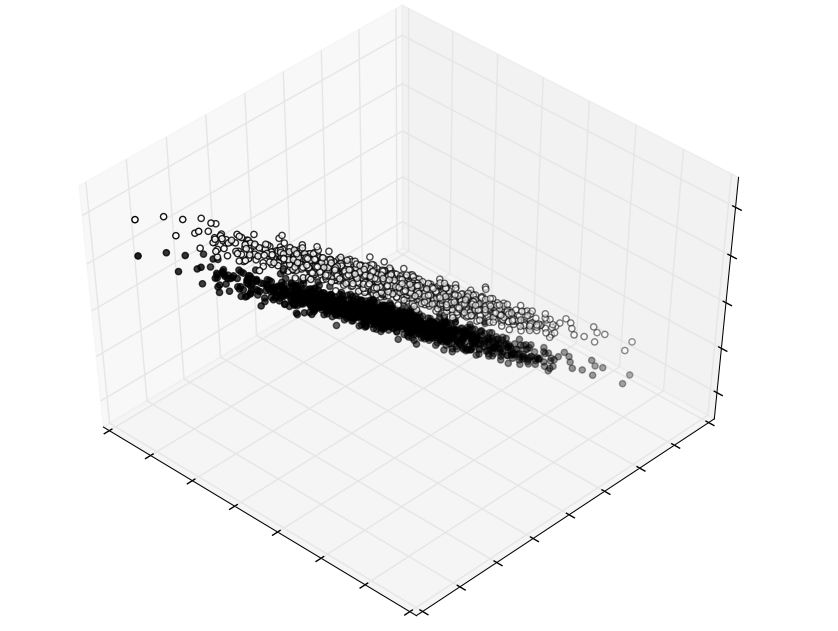
\includegraphics[scale=0.55]{plot_feature_extraction_3d}

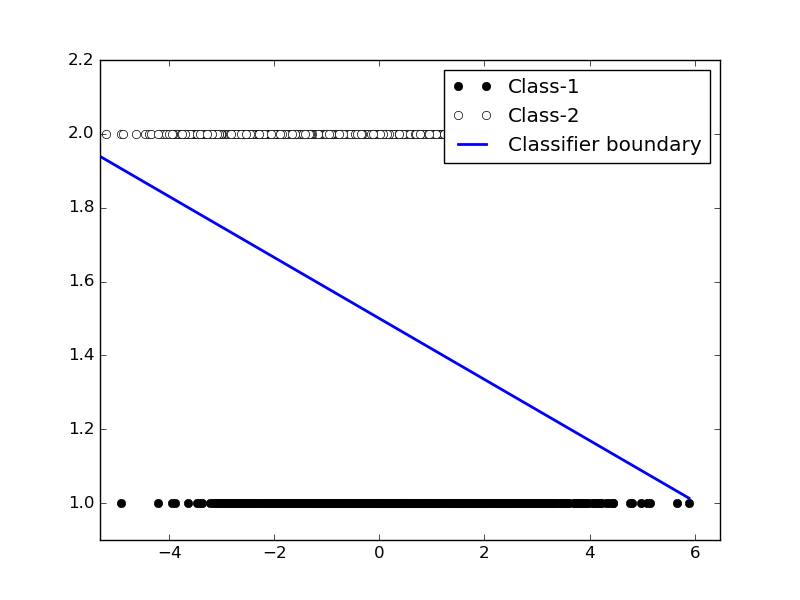
\includegraphics[scale=0.6]{plot_feature_extraction_pca}

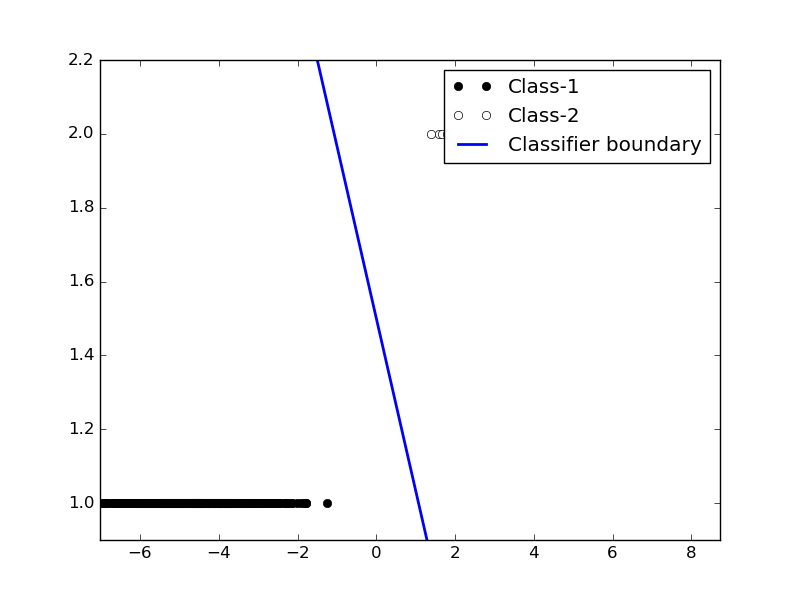
\includegraphics[scale=0.6]{plot_feature_extraction_lda}

\section{Logistic Regression}

\subsection{Goal}

From the given dataset ( called DS2 ) which consists of a number of
images of different categories, we need to perform a 2-class logistic
regression on it, by extracting features from it. Performance using
both L1 and L2 penalty is analysed and reported.

\subsection{Approach}

\subsection{Results}

For L2 penalty, we get the following results.\\

\begin{tabular}{|c|c|c|}
\hline 
Measure & Class - 1 & Class - 2\tabularnewline
\hline 
\hline 
Accuracy & \multicolumn{2}{c|}{52.5 \%}\tabularnewline
\hline 
Precision & 52.0 \% & 53.33 \%\tabularnewline
\hline 
Recall & 65.0 \% & 40.0 \%\tabularnewline
\hline 
F-measure & 0.5778 & 0.0457\tabularnewline
\hline 
\end{tabular}\\
\\
For L1 penalty, we get the following results.\\

\begin{tabular}{|c|c|c|}
\hline 
Measure & Class - 1 & Class - 2\tabularnewline
\hline 
\hline 
Accuracy & \multicolumn{2}{c|}{57.5 \%}\tabularnewline
\hline 
Precision & 56.52 \% & 58.82 \%\tabularnewline
\hline 
Recall & 65.0 \% & 50.0 \%\tabularnewline
\hline 
F-measure & 0.6046 & 0.5405\tabularnewline
\hline 
\end{tabular}\\
\\
We see that, L1 regularised logistic regression performs better than
L2 regularised logistic regression and we have obtained higher accruacy,
precision, recall and F-measure in the former case.

\section{Naive Bayes Classifier}
\end{document}
